\documentclass[12pt,]{article}
\usepackage{lmodern}
\usepackage{amssymb,amsmath}
\usepackage{ifxetex,ifluatex}
\usepackage{fixltx2e} % provides \textsubscript
\ifnum 0\ifxetex 1\fi\ifluatex 1\fi=0 % if pdftex
  \usepackage[T1]{fontenc}
  \usepackage[utf8]{inputenc}
\else % if luatex or xelatex
  \ifxetex
    \usepackage{mathspec}
  \else
    \usepackage{fontspec}
  \fi
  \defaultfontfeatures{Ligatures=TeX,Scale=MatchLowercase}
\fi
% use upquote if available, for straight quotes in verbatim environments
\IfFileExists{upquote.sty}{\usepackage{upquote}}{}
% use microtype if available
\IfFileExists{microtype.sty}{%
\usepackage{microtype}
\UseMicrotypeSet[protrusion]{basicmath} % disable protrusion for tt fonts
}{}
\usepackage[margin=1in]{geometry}
\usepackage{hyperref}
\hypersetup{unicode=true,
            pdftitle={Senegal HIV model},
            pdfauthor={Fabricia F. Nascimento},
            pdfborder={0 0 0},
            breaklinks=true}
\urlstyle{same}  % don't use monospace font for urls
\usepackage{graphicx,grffile}
\makeatletter
\def\maxwidth{\ifdim\Gin@nat@width>\linewidth\linewidth\else\Gin@nat@width\fi}
\def\maxheight{\ifdim\Gin@nat@height>\textheight\textheight\else\Gin@nat@height\fi}
\makeatother
% Scale images if necessary, so that they will not overflow the page
% margins by default, and it is still possible to overwrite the defaults
% using explicit options in \includegraphics[width, height, ...]{}
\setkeys{Gin}{width=\maxwidth,height=\maxheight,keepaspectratio}
\IfFileExists{parskip.sty}{%
\usepackage{parskip}
}{% else
\setlength{\parindent}{0pt}
\setlength{\parskip}{6pt plus 2pt minus 1pt}
}
\setlength{\emergencystretch}{3em}  % prevent overfull lines
\providecommand{\tightlist}{%
  \setlength{\itemsep}{0pt}\setlength{\parskip}{0pt}}
\setcounter{secnumdepth}{0}
% Redefines (sub)paragraphs to behave more like sections
\ifx\paragraph\undefined\else
\let\oldparagraph\paragraph
\renewcommand{\paragraph}[1]{\oldparagraph{#1}\mbox{}}
\fi
\ifx\subparagraph\undefined\else
\let\oldsubparagraph\subparagraph
\renewcommand{\subparagraph}[1]{\oldsubparagraph{#1}\mbox{}}
\fi

%%% Use protect on footnotes to avoid problems with footnotes in titles
\let\rmarkdownfootnote\footnote%
\def\footnote{\protect\rmarkdownfootnote}

%%% Change title format to be more compact
\usepackage{titling}

% Create subtitle command for use in maketitle
\newcommand{\subtitle}[1]{
  \posttitle{
    \begin{center}\large#1\end{center}
    }
}

\setlength{\droptitle}{-2em}
  \title{Senegal HIV model}
  \pretitle{\vspace{\droptitle}\centering\huge}
  \posttitle{\par}
  \author{Fabricia F. Nascimento}
  \preauthor{\centering\large\emph}
  \postauthor{\par}
  \predate{\centering\large\emph}
  \postdate{\par}
  \date{2018-06-27}

\usepackage{booktabs}
\usepackage{longtable}
\usepackage{array}
\usepackage{multirow}
\usepackage[table]{xcolor}
\usepackage{wrapfig}
\usepackage{float}
\usepackage{colortbl}
\usepackage{pdflscape}
\usepackage{tabu}
\usepackage{threeparttable}
\usepackage[normalem]{ulem}

\begin{document}
\maketitle

\hypertarget{introduction}{%
\section{Introduction}\label{introduction}}

\begin{itemize}
\tightlist
\item
  Phylogenetic trees were estimated using the RaxML for each HIV-1
  subtype: C and 02\_AG;
\item
  Using information on when sequences were collected, a phylogenetic
  tree, in which branch length were in units of calendar times, were
  also estimated using treedater;
\item
  These dated phylogenetic trees were analysed in separate;
\item
  Each tip of the pylogenetic tree was associated to a state (see
  section below);
\item
  If a tip could not be associated to a state (because of missing
  information in the metadata), this particular tip was removed from the
  dated tree;
\item
  The dated phylogenetic tree for each subtype in which all tips could
  be assigned to a state were then used with phydynR to estimate the
  transmission rates and parameters of the model (see below for more
  information on which parameters we are estimating).
\end{itemize}

\hypertarget{the-model}{%
\section{The Model}\label{the-model}}

The model we fit is based on the structured coalescent models (Volz
2012). These models are used to estimate epidemiological parameters
using a phylogenetic tree and information on states of each tip of the
tree. These states are discrete-trait information representing each
sequence.

In our mathematical model we have 4 different discrete-traits associated
to each DNA sequence:

\begin{itemize}
\tightlist
\item
  \(gpf\) = infected heterosexual females from the general population;
\item
  \(gpm\) = infected heterosexual males from the general population;
\item
  \(msm\) = infected male that have sex with other men;
\item
  \(src\) = source sample, which are infected individuals that are from
  other countries and not from Senegal.
\end{itemize}

\hypertarget{stage-of-infection}{%
\subsection{Stage of infection}\label{stage-of-infection}}

We fit the HIV epidemic in Senegal using ordinary differential equations
(ODE) and only 1 stage of infection. This means that infected
individuals would die and not recover from the infection. In our model
we represented it as \(\gamma\) rate. We used 1 stage of infection,
because the metadata available for the Senegal sequences did not have
information that we could use to determine the stage of HIV infection at
the time the samples were collected.

\hypertarget{how-transmissions-were-modelled}{%
\subsection{How transmissions were
modelled?}\label{how-transmissions-were-modelled}}

\begin{itemize}
\tightlist
\item
  An infected \(msm\) (\(I_{msm}\)) could transmite to another \(msm\)
  with probability \(p_{msm2msm}\)
\item
  An infected \(msm\) (\(I_{msm}\)) could transmit to a \(gpf\) with
  probability \((1 - p_{msm2msm})\)
\item
  An infected \(gpf\) (\(I_{gpf}\)) could transmit to a \(gpm\) with
  probability \(p_{gpf2gpm}\)
\item
  An infected \(gpf\) (\(I_{gpf}\)) could transmit to a \(msm\) with
  probability \((1 - p_{gpf2gpm})\)
\item
  An infected \(gpm\) (\(I_{gpm}\)) could also transmit to a \(gpf\).
  This is the risk ratio of a male (\(gpm\)) to transmite to a female
  (\(gpf\)). This is the parameter \(male_{x}\) of our model.
\end{itemize}

See Figure 1 for a partil schematic representation of the transmission
model for HIV in Senegal. In this figure \(gpf\), \(gpm\) and \(msm\)
represent the infected individuals.

\begin{figure}[H]

{\centering 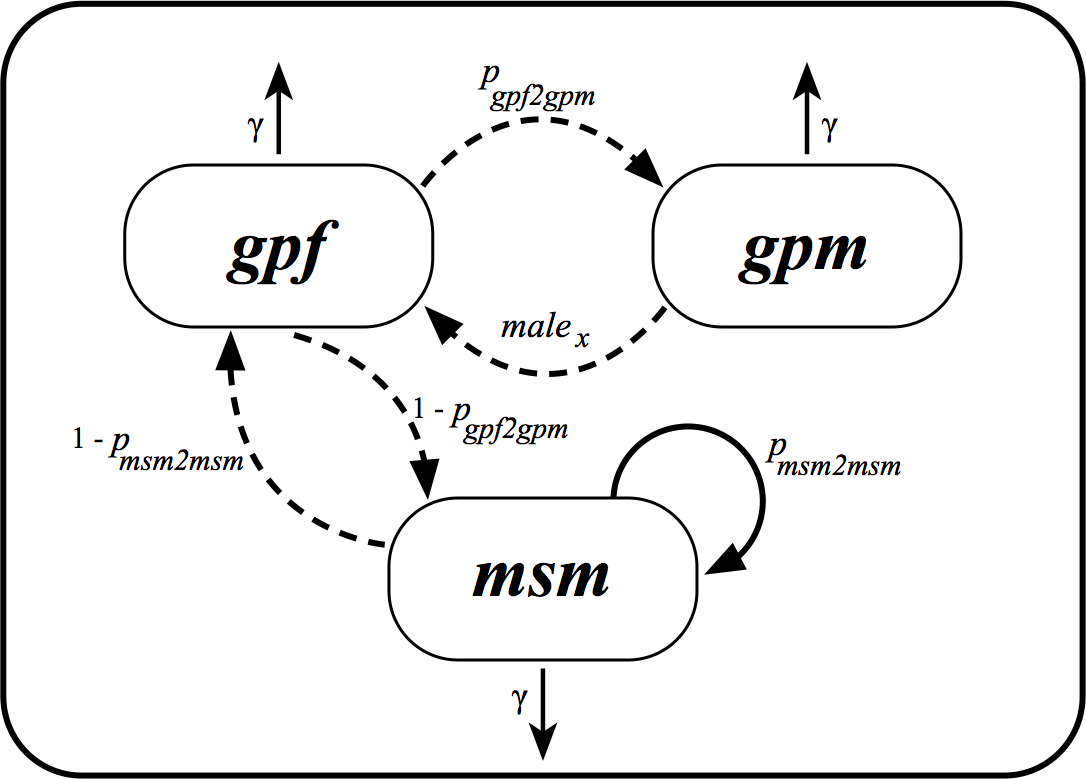
\includegraphics[width=0.9\linewidth]{images/SN_model_v3} 

}

\caption{Transmission model for HIV in Senegal. $gpf$, $gpm$ and $msm$ represent infected individuals.}\label{fig:unnamed-chunk-1}
\end{figure}

\hypertarget{how-about-hiv-incidence-rate}{%
\subsection{How about HIV incidence
rate?}\label{how-about-hiv-incidence-rate}}

We also modelled the HIV incidence rate as a funtion of time (\(t\)) in
\(msm\) and the \(gp\) (general population) as different spline
functions (Eilers and Marx 1996), that in our ODEs are represented by
\(\lambda(t)\) and \(\mu(t)\), respectively.

\hypertarget{the-source-compartment}{%
\subsection{\texorpdfstring{The \(source\)
compartment}{The source compartment}}\label{the-source-compartment}}

Finally, to model the HIV epidemic in Senegal, we also added an
additional compartment named ``source'' (\(src\)), that represents the
rate in which HIV lineages are imported to Senegal from other countries.
We modelled this as a constant efective population size rate with two
parameters to be estimeted -- \(srcNe\): the effective source population
size; and the \(import\) rate. Because the number of imported HIV
balances the number of exported HIV, the infected \(src\) individuals
along time are not represented in the ODEs.

\hypertarget{the-odes-or-mathematical-model-equations}{%
\subsection{The ODEs or mathematical model
equations}\label{the-odes-or-mathematical-model-equations}}

\(\dot{I}_{gpf} = male_x \mu(t) I_{gpm} + (1 - p_{msm2msm}) \lambda(t) I_{msm} - \gamma I_{gpf}\)

\(\dot{I}_{gpm} = p_{gpf2gpm} \mu(t) I_{gpf} - \gamma I_{gpm}\)

\(\dot{I}_{msm} = (1 - p_{gpf2gpm}) \mu(t) I_{gpf} + p_{msm2msm} \lambda(t) I_{msm} - \gamma I_{msm}\)

\hypertarget{estimation-of-epidemiological-parameters}{%
\section{Estimation of epidemiological
parameters}\label{estimation-of-epidemiological-parameters}}

For the Senegal HIV model, we are estimating the parameters using a
Markov chain Monte Carlo (MCMC) as implemented in the R package
\href{\%22https://github.com/florianhartig/BayesianTools\%22}{BayesianTools}.

\hypertarget{parameters-to-be-estimated-and-priors}{%
\subsection{Parameters to be estimated and
priors}\label{parameters-to-be-estimated-and-priors}}

\textbf{Parameters for estimating the spline function for the
\emph{gp}:}

\begin{itemize}
\tightlist
\item
  \emph{gpsp0}: prior chosen in order to have the mean of \(R_0 = 1.1\)
\item
  \emph{gpsp1}: prior chosen in order to have the mean of \(R_0 = 1.1\)
\item
  \emph{gpsp2}: prior chosen in order to have the mean of \(R_0 = 1.1\)
\item
  \emph{gpsploc}
\end{itemize}

\textbf{Parameters for estimating the spline function for the
\emph{msm}:}

\begin{itemize}
\tightlist
\item
  \emph{msmsp0}: prior chosen in order to have the mean of \(R_0 = 1.1\)
\item
  \emph{msmsp1}: prior chosen in order to have the mean of \(R_0 = 1.1\)
\item
  \emph{msmsp2}: prior chosen in order to have the mean of \(R_0 = 1.1\)
\item
  \emph{msmsploc}
\end{itemize}

Note that the spline shape parameters (\emph{gpsp0}, \emph{gpsp1},
\emph{gpsp2}, \emph{msmsp0}, \emph{msmsp1}, \emph{msmsp2}) represent the
number of transmissions per infected individual.

Given the equation for R\_0, we have:

\(R_0 = \beta/\gamma\)

In our model \(\gamma = 0.1\), and \(\beta\) will be represented by each
of the spline shape parameters. We are aiming to have a curve
representing the number of tansmissions per infected individuals

\textbf{Parameters that controls the \emph{src}:}

\begin{itemize}
\tightlist
\item
  \emph{import}: prior chosen with mean around \(0.03\)
\item
  \emph{srcNe}: prior chosen with mean around \(100\)
\end{itemize}

\textbf{Probability of certain events to occour:}

\begin{itemize}
\tightlist
\item
  \emph{pmsm2msm} : prior chosen with mean around \(0.80\)
\item
  \emph{pgpf2gpm} : prior chosen with mean around \(0.80\)
\end{itemize}

\textbf{Initial population sizes:}

\begin{itemize}
\tightlist
\item
  \emph{initgp}: prior chosen with mean around \(3\)
\item
  \emph{initmsm}: prior chosen with mean around \(3\)
\end{itemize}

See Table 1 for a list of parameters that we are estimating and the
priors used. Note that lower and upper bounds for the priors were used
to keep the posterior distribution at sensible values when using the
BayesianTools R package. If such bounds were not provided negative or
very high values, when low values were expected, could be proposed
during the MCMC.

\rowcolors{2}{gray!6}{white}
\begin{table}[!h]

\caption{\label{tab:unnamed-chunk-2}Parameter definition, symbols used in the ODEs, priors with lower and upper bounds}
\centering
\resizebox{\linewidth}{!}{\begin{tabular}[t]{lllll}
\hiderowcolors
\toprule
Parameter & Symbol in R & Prior & Lower & Upper\\
\midrule
\showrowcolors
Spline shape gp0 & gpsp0 & Gamma(3, 3/0.1) & 0.05 & 1\\
Spline shape gp1 & gpsp1 & Gamma(3, 3/0.1) & 0.05 & 1\\
Spline shape gp2 & gpsp2 & Gamma(3, 3/0.1) & 0.05 & 1\\
Spline interval gp & gpsploc & U(1978, 2014) & 1978 & 2014\\
Spline shape msm0 & msmsp0 & Gamma(3, 3/0.1) & 0.05 & 1\\
\addlinespace
Spline shape msm1 & msmsp1 & Gamma(3, 3/0.1) & 0.05 & 1\\
Spline shape msm2 & msmsp2 & Gamma(3, 3/0.1) & 0.05 & 1\\
Spline interval msm & msmsploc & U(1978, 2014) & 1978 & 2014\\
Infectiouness ratio from male to female & maleX & U(0.5, 2) & 0.5 & 10\\
Importation rate & import & Exp(30) & 0 & 0.30\\
\addlinespace
Effective population size of src & srcNe & Exp(1/100) & 1 & 5000\\
Probability of infected msm to infect another msm & pmsm2msm & Beta(16, 4) & 0 & 1\\
Probability of infected gpf to infect a gpm & pgpf2gpm & Beta(16, 4) & 0 & 1\\
Initial number of infected msm & initmsm & Exp(1/3) & 1 & 300\\
Initial number of infected gp & initgp & Exp(1/3) & 1 & 300\\
\bottomrule
\end{tabular}}
\end{table}
\rowcolors{2}{white}{white}

\hypertarget{partial-results}{%
\section{Partial results}\label{partial-results}}

\begin{itemize}
\item
  A total of 116 and 355 sequences were analysed for subtype C and
  02\_AG, respectively (including sequences that were not from Senegal,
  to represent the source compartment). From those, 100 and 302 are
  sequences from Senegal, respectively.
\item
  After fitting the mathematical model to the phylogenetic tree, we can
  calculate the effective number of infections, the number of new cases,
  and PAF (proportion attributable fraction of transmissions), as
  exemplified in the plots for subtypes C and 02\_AG. Note that in each
  plot the solid line is the median and the dashed line is the MAP
  (maximum a posteriori).
\end{itemize}

\hypertarget{parameter-of-interest}{%
\subsection{Parameter of interest}\label{parameter-of-interest}}

Below is a table showing the estimated value for a parameter of
interest: \emph{pmsm2msm}

\rowcolors{2}{gray!6}{white}
\begin{table}[!h]

\caption{\label{tab:unnamed-chunk-3}Median, MAP, 
                             and credible interval for parameter $pmsm2msm$ as estimated by our model}
\centering
\begin{tabu} to \linewidth {>{\raggedright}X>{\raggedright}X>{\raggedright}X>{\raggedright}X>{\raggedright}X}
\hiderowcolors
\toprule
Parameter & Median & MAP & 2.5\% & 97.5\%\\
\midrule
\showrowcolors
C & 0.842 & 0.869 & 0.721 & 0.923\\
02\_AG & 0.848 & 0.899 & 0.706 & 0.949\\
\bottomrule
\end{tabu}
\end{table}
\rowcolors{2}{white}{white}

\hypertarget{some-thoughts-about-the-results}{%
\subsection{Some thoughts about the
results}\label{some-thoughts-about-the-results}}

Results observed by subtype are very different, and we think this is
because the way samples were sampled were not random, and the
distribution of subtypes C and 02\_AG differs between the heterosexual
general population and msm. For example: 40\% of msm in Senegal are
infected with subtype C, while only 4-10\% infects general population
and FSW (female sex workers) (Ndiaye et al. 2009, 2013).

In the general population, the picture is different, and subtype 02\_AG
infects 64\% of the general population (Ndiaye et al. 2013).

These observations could reflect the different results observed by the
different HIV subtypes.

\hypertarget{references}{%
\section*{References}\label{references}}
\addcontentsline{toc}{section}{References}

\hypertarget{refs}{}
\leavevmode\hypertarget{ref-Eilers1996}{}%
Eilers, Paul H C, and Brian D Marx. 1996. ``Flexible smoothing with
B-splines and penalties.'' \emph{Statistical Science} 11 (2):89--121.
\url{https://doi.org/10.1214/ss/1038425655}.

\leavevmode\hypertarget{ref-Ndiaye2013}{}%
Ndiaye, Halimatou Diop, Edmond Tchiakpe, Nicole Vidal, Ousseynou Ndiaye,
Abdou Khoudia Diop, Martine Peeters, Souleymane Mboup, and Coumba
Toure-Kane. 2013. ``HIV type 1 subtype C remains the predominant subtype
in men having sex with men in Senegal.'' \emph{AIDS Research and Human
Retroviruses}. \url{https://doi.org/10.1089/aid.2013.0140}.

\leavevmode\hypertarget{ref-Ndiaye2009}{}%
Ndiaye, Halimatou Diop, Coumba Toure-Kane, Nicole Vidal, Fabien Roch
Niama, Pape Amadou Niang-Diallo, Tandakha Dièye, Aissatou Gaye-Diallo,
Abdoulaye Sidibe Wade, Martine Peeters, and Souleymane Mboup. 2009.
``Surprisingly high prevalence of subtype C and specific HIV-1
subtype/CRF distribution in men having sex with men in Senegal.''
\emph{Journal of Acquired Immune Deficiency Syndromes}.
\url{https://doi.org/10.1097/QAI.0b013e3181af70a4}.

\leavevmode\hypertarget{ref-Volz2012}{}%
Volz, Erik M. 2012. ``Complex population dynamics and the coalescent
under neutrality.'' \emph{Genetics} 190 (1):187--201.
\url{https://doi.org/10.1534/genetics.111.134627}.


\end{document}
